\section{Trigger\-Player Class Reference}
\label{classTriggerPlayer}\index{TriggerPlayer@{TriggerPlayer}}
{\bf Trigger}{\rm (p.\,\pageref{classTrigger})} which is passed only by {\bf Player}{\rm (p.\,\pageref{classPlayer})}.  


{\tt \#include $<$triggerplayer.hpp$>$}

Inheritance diagram for Trigger\-Player::\begin{figure}[H]
\begin{center}
\leavevmode
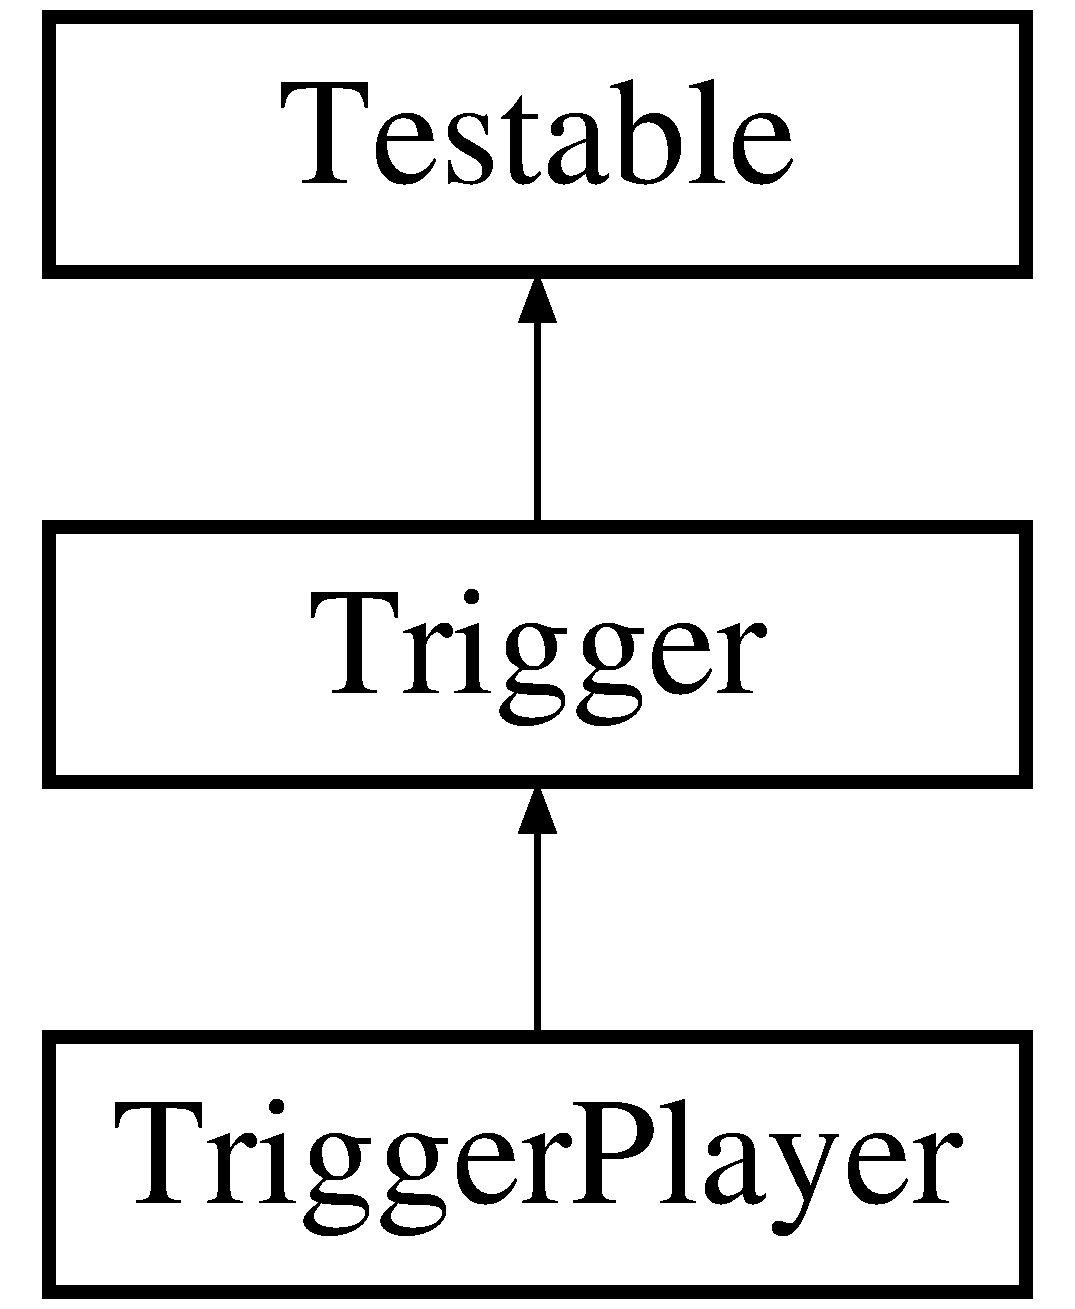
\includegraphics[height=3cm]{classTriggerPlayer}
\end{center}
\end{figure}
\subsection*{Public Member Functions}
\begin{CompactItemize}
\item 
{\bf Trigger\-Player} ()
\item 
{\bf $\sim$Trigger\-Player} ()
\item 
bool {\bf can\-Activate} ({\bf Monster} \&monster)
\item 
QString {\bf name} () const 
\end{CompactItemize}
\subsection*{Protected Member Functions}
\begin{CompactItemize}
\item 
void {\bf cust\-Load} ({\bf Parser} \&parser)
\item 
void {\bf cust\-Save} (ofstream \&file) const 
\end{CompactItemize}


\subsection{Detailed Description}
{\bf Trigger}{\rm (p.\,\pageref{classTrigger})} which is passed only by {\bf Player}{\rm (p.\,\pageref{classPlayer})}. 



\subsection{Constructor \& Destructor Documentation}
\index{TriggerPlayer@{Trigger\-Player}!TriggerPlayer@{TriggerPlayer}}
\index{TriggerPlayer@{TriggerPlayer}!TriggerPlayer@{Trigger\-Player}}
\subsubsection{\setlength{\rightskip}{0pt plus 5cm}{\bf Trigger\-Player} ()}\label{classTriggerPlayer_a0}


\index{TriggerPlayer@{Trigger\-Player}!~TriggerPlayer@{$\sim$TriggerPlayer}}
\index{~TriggerPlayer@{$\sim$TriggerPlayer}!TriggerPlayer@{Trigger\-Player}}
\subsubsection{\setlength{\rightskip}{0pt plus 5cm}$\sim${\bf Trigger\-Player} ()}\label{classTriggerPlayer_a1}




\subsection{Member Function Documentation}
\index{TriggerPlayer@{Trigger\-Player}!canActivate@{canActivate}}
\index{canActivate@{canActivate}!TriggerPlayer@{Trigger\-Player}}
\subsubsection{\setlength{\rightskip}{0pt plus 5cm}bool can\-Activate ({\bf Monster} \& {\em monster})\hspace{0.3cm}{\tt  [virtual]}}\label{classTriggerPlayer_a2}




Implements {\bf Trigger} {\rm (p.\,\pageref{classTrigger_a5})}.\index{TriggerPlayer@{Trigger\-Player}!custLoad@{custLoad}}
\index{custLoad@{custLoad}!TriggerPlayer@{Trigger\-Player}}
\subsubsection{\setlength{\rightskip}{0pt plus 5cm}void cust\-Load ({\bf Parser} \& {\em parser})\hspace{0.3cm}{\tt  [protected, virtual]}}\label{classTriggerPlayer_b0}




Implements {\bf Trigger} {\rm (p.\,\pageref{classTrigger_b0})}.\index{TriggerPlayer@{Trigger\-Player}!custSave@{custSave}}
\index{custSave@{custSave}!TriggerPlayer@{Trigger\-Player}}
\subsubsection{\setlength{\rightskip}{0pt plus 5cm}void cust\-Save (ofstream \& {\em file}) const\hspace{0.3cm}{\tt  [protected, virtual]}}\label{classTriggerPlayer_b1}




Implements {\bf Trigger} {\rm (p.\,\pageref{classTrigger_b1})}.\index{TriggerPlayer@{Trigger\-Player}!name@{name}}
\index{name@{name}!TriggerPlayer@{Trigger\-Player}}
\subsubsection{\setlength{\rightskip}{0pt plus 5cm}QString name () const\hspace{0.3cm}{\tt  [virtual]}}\label{classTriggerPlayer_a3}




Implements {\bf Trigger} {\rm (p.\,\pageref{classTrigger_a7})}.

The documentation for this class was generated from the following files:\begin{CompactItemize}
\item 
{\bf triggerplayer.hpp}\item 
{\bf triggerplayer.cpp}\end{CompactItemize}
